\section{Entwicklung eines Konzepts für die Verifizierung und das Labeln der Ereignisse} \label{sec:Meth Labeling}
Da die Modellauswahl eingegrenzt wurde auf Modelle des überwachten Lernens, werden gelabelte Ereignisse benötigt. Dafür ist ein Konzept zu erstellen. Grundlage für das Labeln ist ein Datensatz mit herausgesuchten Ereignissen. Das Heraussuchen erfolgte bereits vor dieser Arbeit. Diese herausgesuchten Ereignisse sind mit einem Label, einem Datum der Startuhrzeit und der Enduhrzeit des Ereignisses vermerkt. Die Uhrzeiten sind jedoch nur grob ermittelt. Die Ereignisse sind in einer csv-Datei gespeichert. Genaueres zu diesem Datensatz folgt in  \autoref{sec:Meth Datensatz}. \par

Es ist Wichtig, dass ein Ereignis zeitlich exakt eingegrenzt wird, damit die charakteristischen Merkmale daraus extrahiert werden können. Ebenfalls soll sichergestellt werden, dass in einem angegebenen Zeitraum auch genau diese charakteristischen Merkmale zu sehen sind. Aus diesem Grund sind die herausgesuchten Ereignisse zu Verifizieren und der exakte Zeitraum ist zu bestimmen. \par 

Die Verifizierung erfolgt visuell. Dafür werden die Videos benötigt. In diesen muss ein Ereignis zu sehen sein, damit es verifiziert werden kann. Der exakte Start- und Endzeitpunkt eines Ereignisses muss Markiert werden können. Dazu können die Detektionsdatensätze verwendet werden (\autoref{sec:Meth RohDat}). In diesem ist für jedes Frame ein Zeitstempel vorhanden. Neben dem Zeitstempel befindet sich in den Datensätzen eine Identifikationsnummer jedes Frame. Diese Stimmt mit der Position des Frames im Video überein. Darüber lassen sich die Frames und die Datensatzeinträge zuordnen. Das Verifzizierungsprogramm bekommt somit als Eingabe die Liste mit den herausgesuchten Ereignissen, Videos und die Detektionsdatensätze. Die Videos und die Detektionsdatensätze werden von einem Hilfsmodul übernommen. Dieses sucht basierend auf einer Datums und Zeitpunktangabe die Dateipfade der passenden Videodatei und des passenden Detektionsdatensatzes heraus. Die Ausgabe des Programms wird ein Datensatz mit den verifizierten Ereignissen. In diesem Datensatz ist der exakte Startzeitpunkt und Enzeitpunkt vermerkt, sowie das Label des Ereignisses. Ebenfalls gibt das Programm einen Datensatz aus mit den Ereignissen die sich nicht verifizieren ließen. Die Detektionsdaten müssen aus der Datenbank in eine csv-Datei heruntergeladen werden. Ist dies noch nicht erfolgt, kann ein Ereignis nicht verifiziert werden. Ereignisse mit fehlenden Detektionsdaten oder fehlenden Videos werden ebenfalls in einer Liste vermerkt. Diese Liste kann von einem weiteren Programm gelesen werden, welches versucht die Fehlenden Daten herunterzuladen. Anschließend kann erneut versucht werden, das Ereignis zu verifizieren. Final erstellt das Programm eine Liste mit allen Ereignissen die sich verifizieren ließen. Das Blockdiagramm dieses Konzepts ist in der Abbildung \ref{fig:BlockLabeling} zu sehen. 

\begin{figure}[htbp]
    \centering
    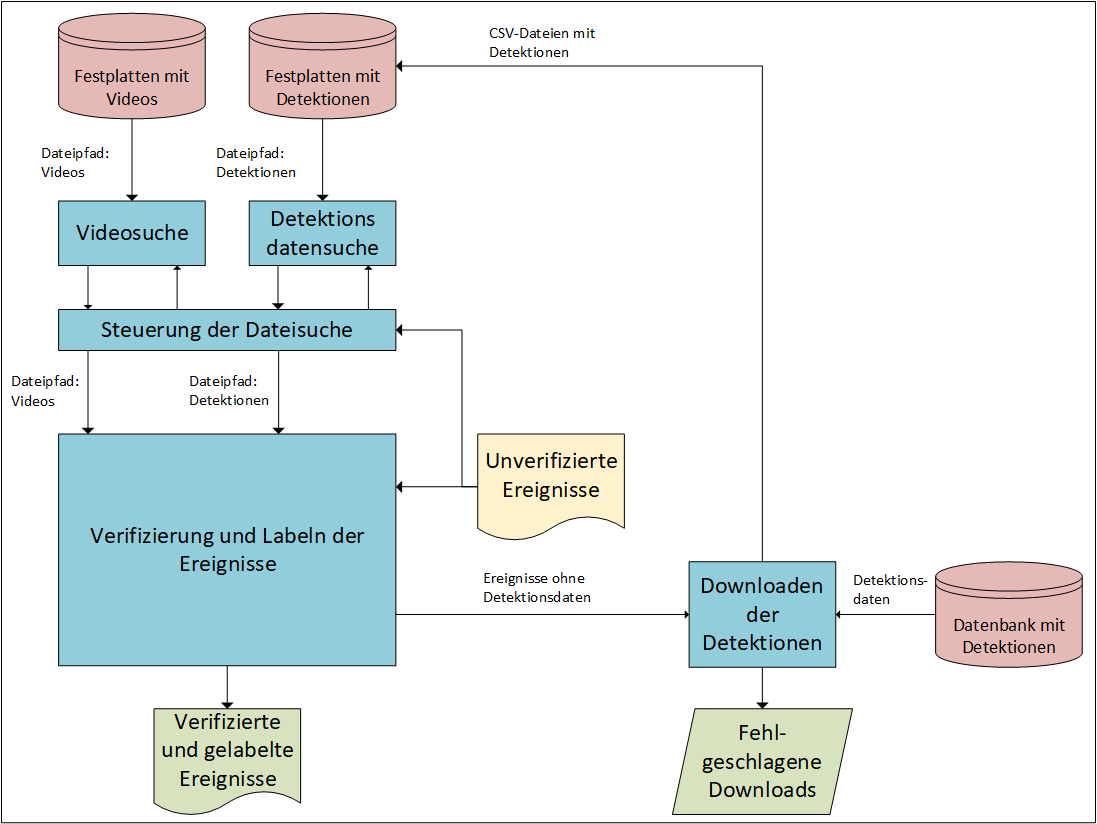
\includegraphics[width=\textwidth]{img/Grafiken/Verifizierungstool Konzept.png}
    \caption[Blockdiagramm des Verifizierungskonzepts.]{Blockdiagramm des Verifizierungskonzepts. Blau dargestellt sind Programmmodule. Die Eingänge sind gelb markiert, Ausgänge sind grün und Speicher sind rot abgebildet.}
    \label{fig:BlockLabeling}
\end{figure}


Wie erwähnt muss die Verifizierung visuell über die Videos erfolgen. Ideal ist es, wenn der Anwender direkt im Video die Zeitpunkte eines Ereignis markieren kann. Dies ist über folgenden Weg möglich. Der Anwender schaut sich das Video an, findet er das zu verifizierende Ereignis, wählt dieser ein Frame als Startframe aus. Über die Position des Frames im Video, wird die Identifikationsnummer des Frames ermittelt. Mit dieser wird der zugehörige Eintrag im Detektionsdatensatz gesucht. Dort ist der Zeitstempel vermerkt. Der Zeitstempel wird als Startzeitpunkt abgespeichert. \par 

Anwenderfreunldich ist auch eine Automatisierung des Prozesses, so dass nicht jedes Ereignis, das zugehörige Video und die Detektionsdaten manuell ausgewählt und herausgesucht werden müssen. Für das heraussuchen der Videos und der Detektionsdatensätze wurden bereits vor dieser Arbeit Programme geschrieben die dies Automatisieren. Lediglich ein Datum und ein Zeitpunkt wird benötigt, um die entsprechenden Dateien herauszusuchen. Da die Ereignisse in einer csv-Datei abgelegt sind, können diese iterativ Aufgerufen werden. So ist der gesamte Ablauf automatisierbar. \par

Das Programm zum herunterladen der Detektionsdaten entstand ebenfalls bereits vor dieser Arbeit und ließ sich leicht in das Konzept Integrieren. 